\section{Hello World}
\label{sec.hello.world}

The first program we usually write in any programming language is
called \code{hello-world}.  It is a very simple program.  However
getting it to run means you have to understand how to use the
programming environment.

\subsection{Examine the Code}
\label{sec.examine.the.code}
Take a look at the Python code in the file \code{src/hello.py}.  In
particular there are two sections in the code,
\begin{enumerate}
\item A declaration of the function named \code{hello}, shown in
  Listing~\ref{list.hello}
\item Two conditional calls to the function \code{hello}, each time
  with a different argument, shown in Listing~\ref{list.calls}.
\end{enumerate}

\begin{listing}{Declaration of Function \code{hello}}{hello}
\begin{minipage}[c]{0.95\textwidth}\begin{lstlisting}
def hello(name):
    print("hello " + name + "!")
\end{lstlisting}\end{minipage}\end{listing}

\begin{listing}{Calls to Function \code{hello}}{calls}
\begin{minipage}[c]{0.95\textwidth}\begin{lstlisting}
if __name__ == '__main__':
    # call the function with an argument
    hello("gertrude")
    
    # second test
    hello("fred")
\end{lstlisting}\end{minipage}\end{listing}


\subsection{Make a Sample Run}

Find the icon 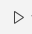
\includegraphics[height=1.0cm]{run-triangle.png} in the
top-right of the editor window.  Click the triangle, to see a sample
run/execution of the code.

\noindent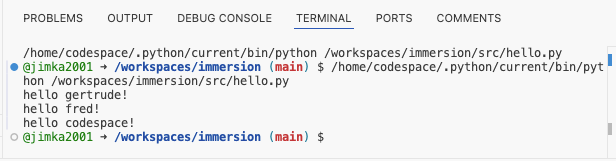
\includegraphics[width=\textwidth]{hello-terminal-output.png}


\subsection{Running Predefined Tests}
\label{sec.run.tests}

Open the file \code{tests/test\_hello.py} in a GitHub Code-Space.

\noindent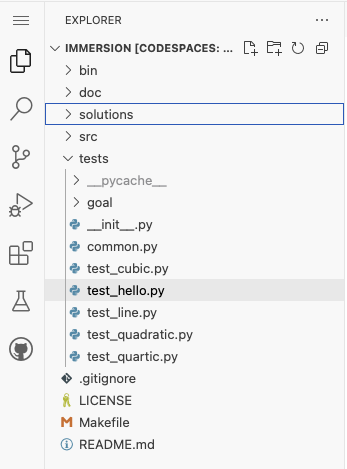
\includegraphics[width=0.4\textwidth]{test-hello-explorer.png}

To run the tests, press the
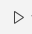
\includegraphics[width=1cm]{run-triangle.png} which you should find in
the upper-right corner of the editor window.

\noindent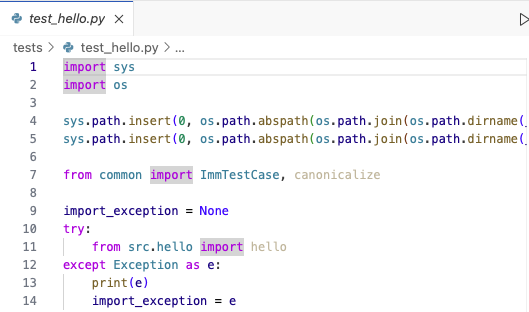
\includegraphics[width=0.8\textwidth]{hello-test.png}


The text window at the bottom of the editor should show the results of
how many tests ran and whether there are any failures.

\noindent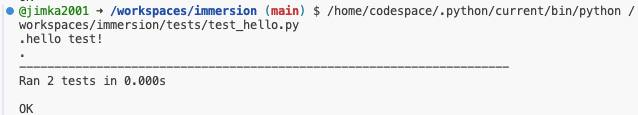
\includegraphics[width=0.9\textwidth]{github-test-result.png}



\subsection{Challenges for the Student}

Understanding errors and debugging is difficult, but it is part of
programming.

Experiment with the simple pieces of code in the above sections.
Insert spaces and press the run button.  Look at the error messages
produced. Remove some quotation marks or parentheses (leaving
unbalanced quotations marks or parentheses)---again look at what error
messages you see when you try to run invalid code.


\begin{enumerate}
\item Remove and add some spaces at the beginning of a line.
\item Change the indentation.
\item Unbalance the parentheses.
\item Unbalance the quotation marks.
\item Put extra spaces inside the quotation marks.
\item Change the name of the \code{hello} function at definition site
  or call site.
\item Figure out how to undo your changes in the editor to make the
  code work again.
\item Run the tests \code{test/test\_hello.py} as explained in
  Section~\ref{sec.run.tests}.
\end{enumerate}

\clearpage
